\documentclass[12pt,UTF8,a4paper]{ctexart}
\usepackage[margin=2.5cm]{geometry}
\usepackage{graphicx}
\graphicspath{{figures/}}
\usepackage{booktabs}
\usepackage{amsmath}
\usepackage{caption}
\usepackage{hyperref}
\captionsetup{font=small}
\DeclareMathOperator*{\argmin}{arg\,min}
\setlength{\parskip}{0.5em}

\title{\textbf{远距机场自主选配、进场规划与切线消高}\\[0.5em]
\large SimplePlanes 2 飞行控制学习项目·SC-3b 验证试验报告（封版版）}
\author{}
\date{2026 年 9 月 23 日初版（v4.48）；9 月 24 日封版后收口（v4.68）}

\begin{document}
\maketitle
\thispagestyle{empty}

\begin{abstract}
本报告记录 SC-3b 课题（任意远距位置单次按键后的全自动进场着陆）的控制架构设计与试飞验证结果。在平台仅提供静态跑道表、无风向接口、无地形数据的约束下，建立了``选配跑道 $\rightarrow$ 进场方式与剖面规划 $\rightarrow$ 直线截获或程序/切线圆消高 $\rightarrow$ FAF 闸门 $\rightarrow$ 定版下滑律''的分级状态机：下滑以下流程与 SC-3 封版律完全一致，进近段的职责被明确界定为在切线点之前把飞机送到规定航道与规定高度。经 v4.18 至 v4.48 共三十余轮迭代、26 个归档架次，末版在 1352 m 高度、9.0 km 距离的山区机场接管中实现切线圆消高、切点零转弯并入、沿中线平飞、截获下滑至接地停稳的全程零人工接管。试验判定主链路验收通过并封版；地形感知、复飞程序重加入等列为遗留项。
\end{abstract}

\section{任务定义与设计约束}
SC-3（近距全自动着陆）封版后，本课题将接管距离从约 2 km 扩展到任意远端：单次按键后，系统需自行选定跑道与方向、规划并飞行进场航段、在规定的入口建立下滑道，其后交接给已封版的着陆链。设计约束有四：

\begin{enumerate}
\item \textbf{机场基准只能用静态表}。跑道头坐标、磁方位与场地标高取自游戏资源包的 Location 文本资产（13 个端头入表）；坐标映射经反编译源码锤实为恒等变换（Latitude$\rightarrow$世界 $z$、Longitude$\rightarrow$世界 $x$，零偏移），并经多机场落地残差复核。
\item \textbf{无风向接口}。运行时风向对脚本不可读（判死），选向只能是几何判据，风修正永久挂账。
\item \textbf{机体机动性有限}。TESTaircraft（E1 发动机，602 hp）可用坡度 $55^\circ$，75 m/s 下转弯半径约 480 m；全油门可持续俯冲角实测上界约 $9.3^\circ$；平飞失配平速度约 60--62 m/s。进场程序必须按此包线设计，不能假设瞬时大角度切入可实现。
\item \textbf{地形仅有高度计}。脚本侧唯一地形感知是相对高度（AGL，读数下限约 1.6--2.0 m），无前视地形数据，山区机场走廊只能靠规则规避。
\end{enumerate}

\section{观测与评估方法}
沿用并扩展 SC-2/SC-3 的量化评估链路：机载 Lua 按 10 Hz 输出 TEL（位姿/操纵面）、APP（进近段 $s$、$\varepsilon$、目标高、实际高、空速、侧偏）、LAND（下滑/滑跑段）、POS（世界坐标）四类流；同场景多机按实例号分列、按时间断流切架次。本课题新增两项判据：其一，接地道面判定按\textbf{本跑道实长}计算（由表内对头配对现算长度：Cochran 2970 m、Bannock 2221 m、Kunimitsu 1056 m），触地点报告区分跑道内（rwy=1）、短头（SHORT OF RWY，含距离）、偏侧（OFF-RWY）与冲出（OVERSHOOT）——早期版本曾以大机场包线为山区短跑道签发合格证，属判据失真；其二，3D 航迹离线重建（分段着色+跑道实体+中线延长线），使进场形状可目视裁决。

\section{跑道选配逻辑（定版）}
候选端头须同时满足四道判据，全部在按键时刻一次判定：
\begin{equation}
\mathrm{sel}=\argmin_{e}\ d_{\mathrm{entry}}(e),
\end{equation}
其中 $d_{\mathrm{entry}}(e)$ 为至端头 $e$ 入口的距离。四道判据为（$\beta_e$ 为入口相对本机的方位、$\psi$ 为航向、$\hat{d}_e$ 为着陆方向单位向量、$\mathbf{thr}_e$ 与 $\mathbf{pos}$ 为跑道头与本机位置）：
\begin{itemize}
\item $|\beta_e-\psi|<90^\circ$：入口位于前方半球；
\item $(\mathbf{thr}_e-\mathbf{pos})\cdot\hat{d}_e>300$ m：跑道头尚未越过（接管后首拍不得触发复飞）；
\item $d_{\mathrm{entry}}(e)\le 15$ km：不跨未知走廊瞎飞；
\item $|\beta_e-\psi|<45^\circ$ 的指向候选优先：飞行员意愿高于就近。
\end{itemize}
无候选时输出拒接并完全不接管（接管即复飞、接管即翻扣的历史事故均源于缺此约束）。第 4 条为两级制：机头指向的机场优先，无指向候选才退回最近——仅按距离派场曾把飞机派向背后端头造成 178° 掉头接管。

\section{进场控制架构（定版 v4.48）}
进近段（stage1）与已封版的下滑段（stage2）职责分离：stage1 的唯一任务是把飞机在切线点之前送上``规定航道 + 规定高度''，stage2 及其后流程对每条跑道完全一致。

\subsection{进场方式与可达性规划（按键时刻一次计算）}
记接管时沿跑道投影距离 $s_0$、侧偏 $l_0$、与跑道夹角 $\varepsilon_0$、高度余量 $\Delta h = \text{alt}_0 - A_{pf}$。直线截获放行条件为
\[
|\varepsilon_0| < 70^\circ,\quad s_0 > 2000\ \text{m},\quad s_0 > 1000 + |\ell_0|/\tan 30^\circ,
\]
其中第三式即截获几何需要量（最大前置角 $30^\circ$ 下的收线距离）。在几何可行之外还须\textbf{能量可达}：$\Delta h \le \tan 10^\circ\cdot(s_0 - s_{pf}) + 50$ m；不可达者不拒接、不静默，而是\textbf{自动降级为程序进场}（盘旋消高）。规划同时生成剖面线
\[
A(s) = A_{pf} + \min\!\big(\tan 10^\circ,\ \tfrac{\Delta h}{s_0 - s_{pf}}\big)\,(s - s_{pf})_+,
\]
进近段目标高逐拍取 $A(s)$（程序模式另以程序高封顶，防止绕圈中被 $s$ 往复拽高拽低），执行环的下沉预算与规划同域放开至 $-V_G\tan 10^\circ$。规划器触钳即上报：不可达判定、降级、剖面坡度均写入日志（PROFILE/UNREACHABLE 行）。

\subsection{程序进场与切线圆消高}
程序进场为三航点矩形（下风起始角 $\rightarrow$ base 拐点 $\rightarrow$ final 汇入点），侧向宽度 $W=2.5R$，转弯由坡度限制器（$55^\circ$ 冻结、$70^\circ$ 强制回平）保证有界。若程序末点复检发现高度仍超下滑律接手能力，进入\textbf{切线圆消高}：以 $(s_{wd},\,S W)$ 为圆心、$W$ 为半径的圆与延长线相切；纯追踪 55° 前置角存在系统性抄近道（稳态半径 $\approx 0.89$ 倍设定值），故目标半径补偿 $\times 1.15$ 使圆真实穿线；入轨经圆的远切点过渡（圆心邻域为旋转导引的奇异点）。高度放到位且经过切点时原地释放，切入截获律——切点处切向即着陆方向，并入零转弯。释放瞬间剖面拍平至程序高，防止旧剖面要求重爬。

\subsection{速度、构型与安全底线}
进近段速度带 65 m/s（程序段 75 m/s，为转弯与爬升购买剩余推力），油门管低速侧、减速板管超速侧，禁止互搏；起落架推迟到下滑段或最后 1.5 km 才放下（带轮飞长程序实测造成 $-4$ m/s 匀速下沉的能量死刑）。安全底线三条：越界未建立自动 GO-AROUND（沿中线爬升脱离）；下滑段 AGL$<25$ m 而距跑道尚远时判定``下滑线被地形吃掉''自动转复飞（山区短条实坠案例催生）；所有大机动按实测掉高斜率预支高度（转弯前置高，出弯回收）。

\section{迭代史：四条主线}
26 个归档架次、账本 25 案，可归纳为四条主线（表~\ref{tab:threads}）。
\begin{table}[htb]\centering\small
\caption{迭代主线与代表案例}
\begin{tabular}{p{2.8cm}p{11.4cm}}
\toprule
主线 & 关键事件 \\
\midrule
闸门与几何 & 咬线死锁（判据与执行器可达域不同域，闸门等待它自己不许存在的高度，干越全场 165 s）；平行巡航（截获角=前置角，侧偏每秒收 1 m）；闸门与截获律定版分工：截获律负责收线，闸门只管线干净。 \\
能量与构型 & 65 m/s 带轮直线平飞实测 $-4$ m/s 匀速下沉（爬升指令物理兑现不了）；放轮推迟+程序段提速至 75 m/s；下沉预算与规划同域（$-5$ m/s 钳位曾使前置高成为纸面数字）。 \\
符号与传感器 & 迎角反约定（$\alpha_{\text{read}}=\gamma-\theta$）；滚转轴系反约定致坡度限制器把每次正确改平翻成满舵加深，两局倒扣——跨符号域分支必须先对一帧实飞数据。 \\
规划诚实性 & 静默接管不可达剖面（干越全场复现）$\rightarrow$ 可达性自检；拒接$\rightarrow$降级方案；拉锯折返（三处 180° 间断）$\rightarrow$ 切线圆（相切=速度连续）；纯追踪稳态偏移$\rightarrow$半径补偿。 \\
\bottomrule
\end{tabular}
\label{tab:threads}
\end{table}

\section{试验结果}
表~\ref{tab:score} 给出各阶段代表架次；图~\ref{fig:app19}--\ref{fig:app26} 为三张 3D 航迹重建。

\begin{table}[htb]\centering\small
\caption{代表架次记分卡（TD 接地、CAP 截获）}
\begin{tabular}{llp{2.6cm}p{6.4cm}}
\toprule
架次 & 场景 & 进场方式 & 结果 \\
\midrule
app5 & 2.2 km 侧偏汇入（v1） & 变前置角截获 & TD 跑道内，全链首次闭环 \\
app19 & 12.6 km、2318 m 侧偏 & direct & TD 46 m/s，rwy=1，零接管 \\
app22 & 1447 m 高接管 & 拒接$\rightarrow$手动 & 建立后 SHORT 1224 m 触地（山区走廊，催生地形保险） \\
app24 & 2448 m/9.6 km & pattern 远端消高 & TD 46 m/s，rwy=1，零接管 \\
app26 & 1352 m/9.0 km 山区条 & 切线圆消高 & 接管第一拍入轨、切点释放、TD 45 m/s，rwy=1，零接管 \\
\bottomrule
\end{tabular}
\label{tab:score}
\end{table}

\begin{figure}[htb]\centering
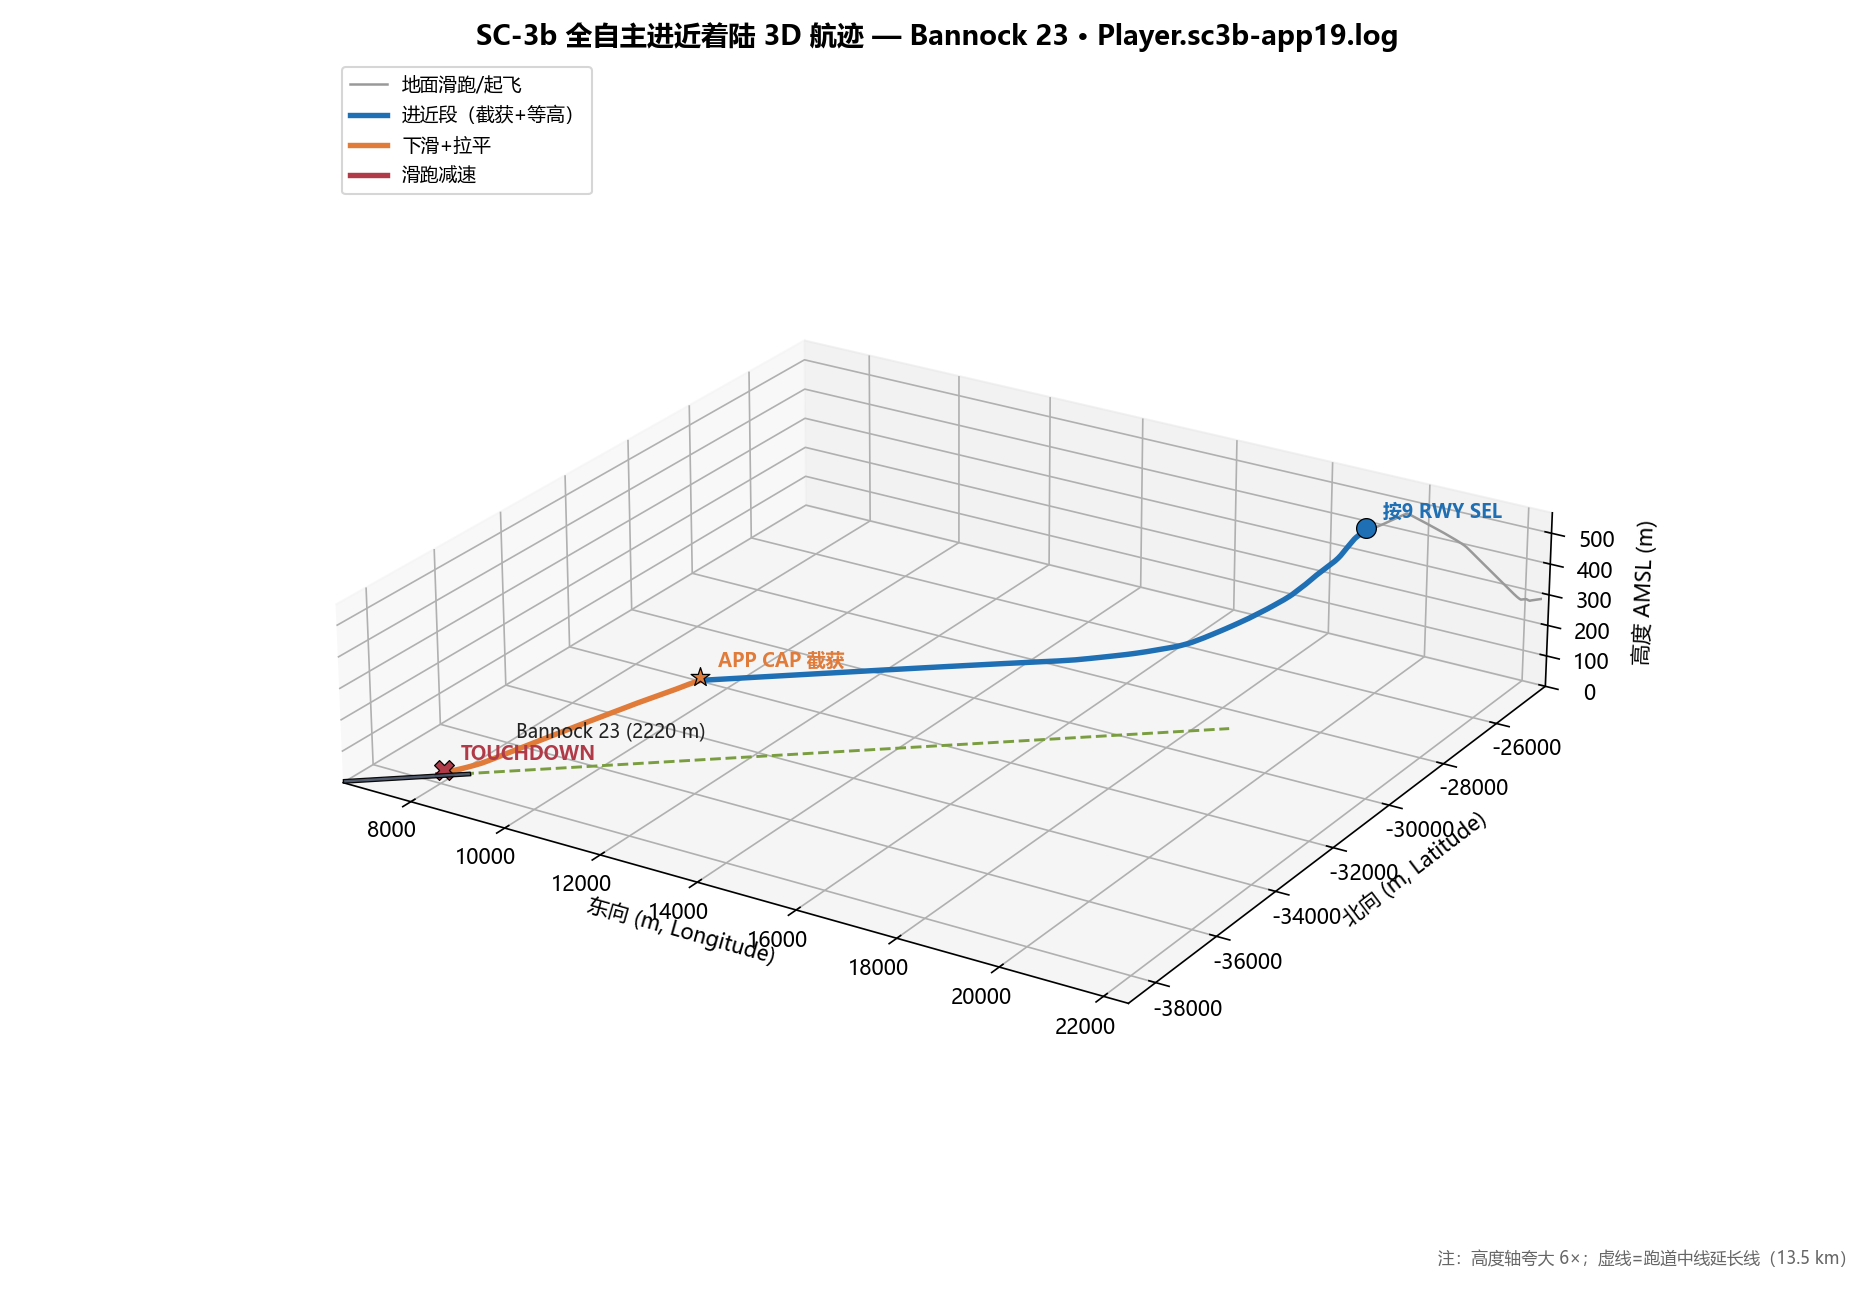
\includegraphics[width=0.98\textwidth]{sc3b-track3d-sc3b-app19.png}
\caption{app19：12.6 km 外直线截获（Bannock 23）。收线 11 km 后 FAF 截获、3.5° 下滑、接地停稳。}\label{fig:app19}
\end{figure}

\begin{figure}[htb]\centering
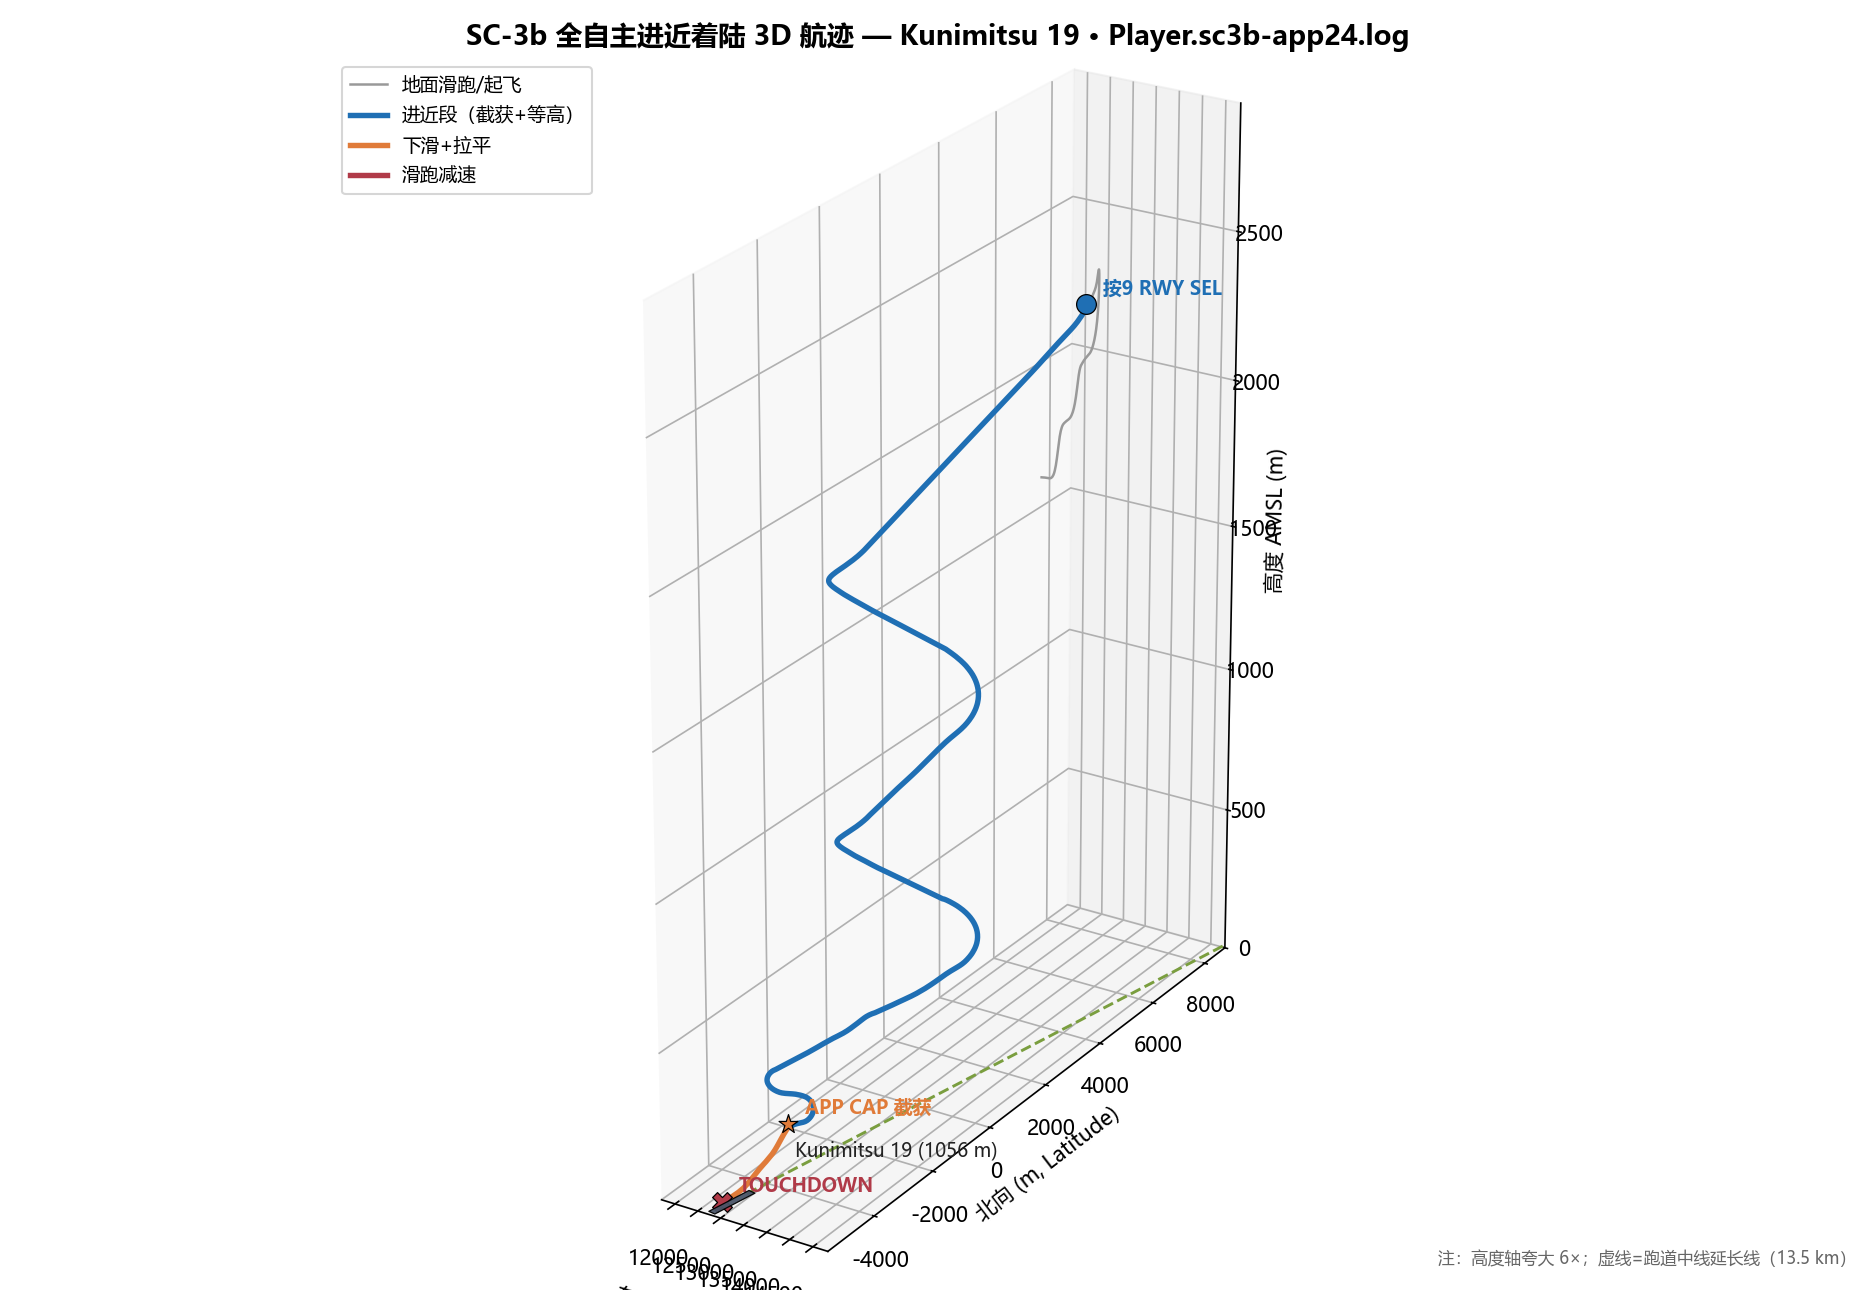
\includegraphics[width=0.98\textwidth]{sc3b-track3d-sc3b-app24.png}
\caption{app24：2448 m 高接管，远端拉锯消高（锯齿形折返，每圈含 180° 间断）后落地——功能闭环、形状欠账，催生切线圆方案。}\label{fig:app24}
\end{figure}

\begin{figure}[htb]\centering
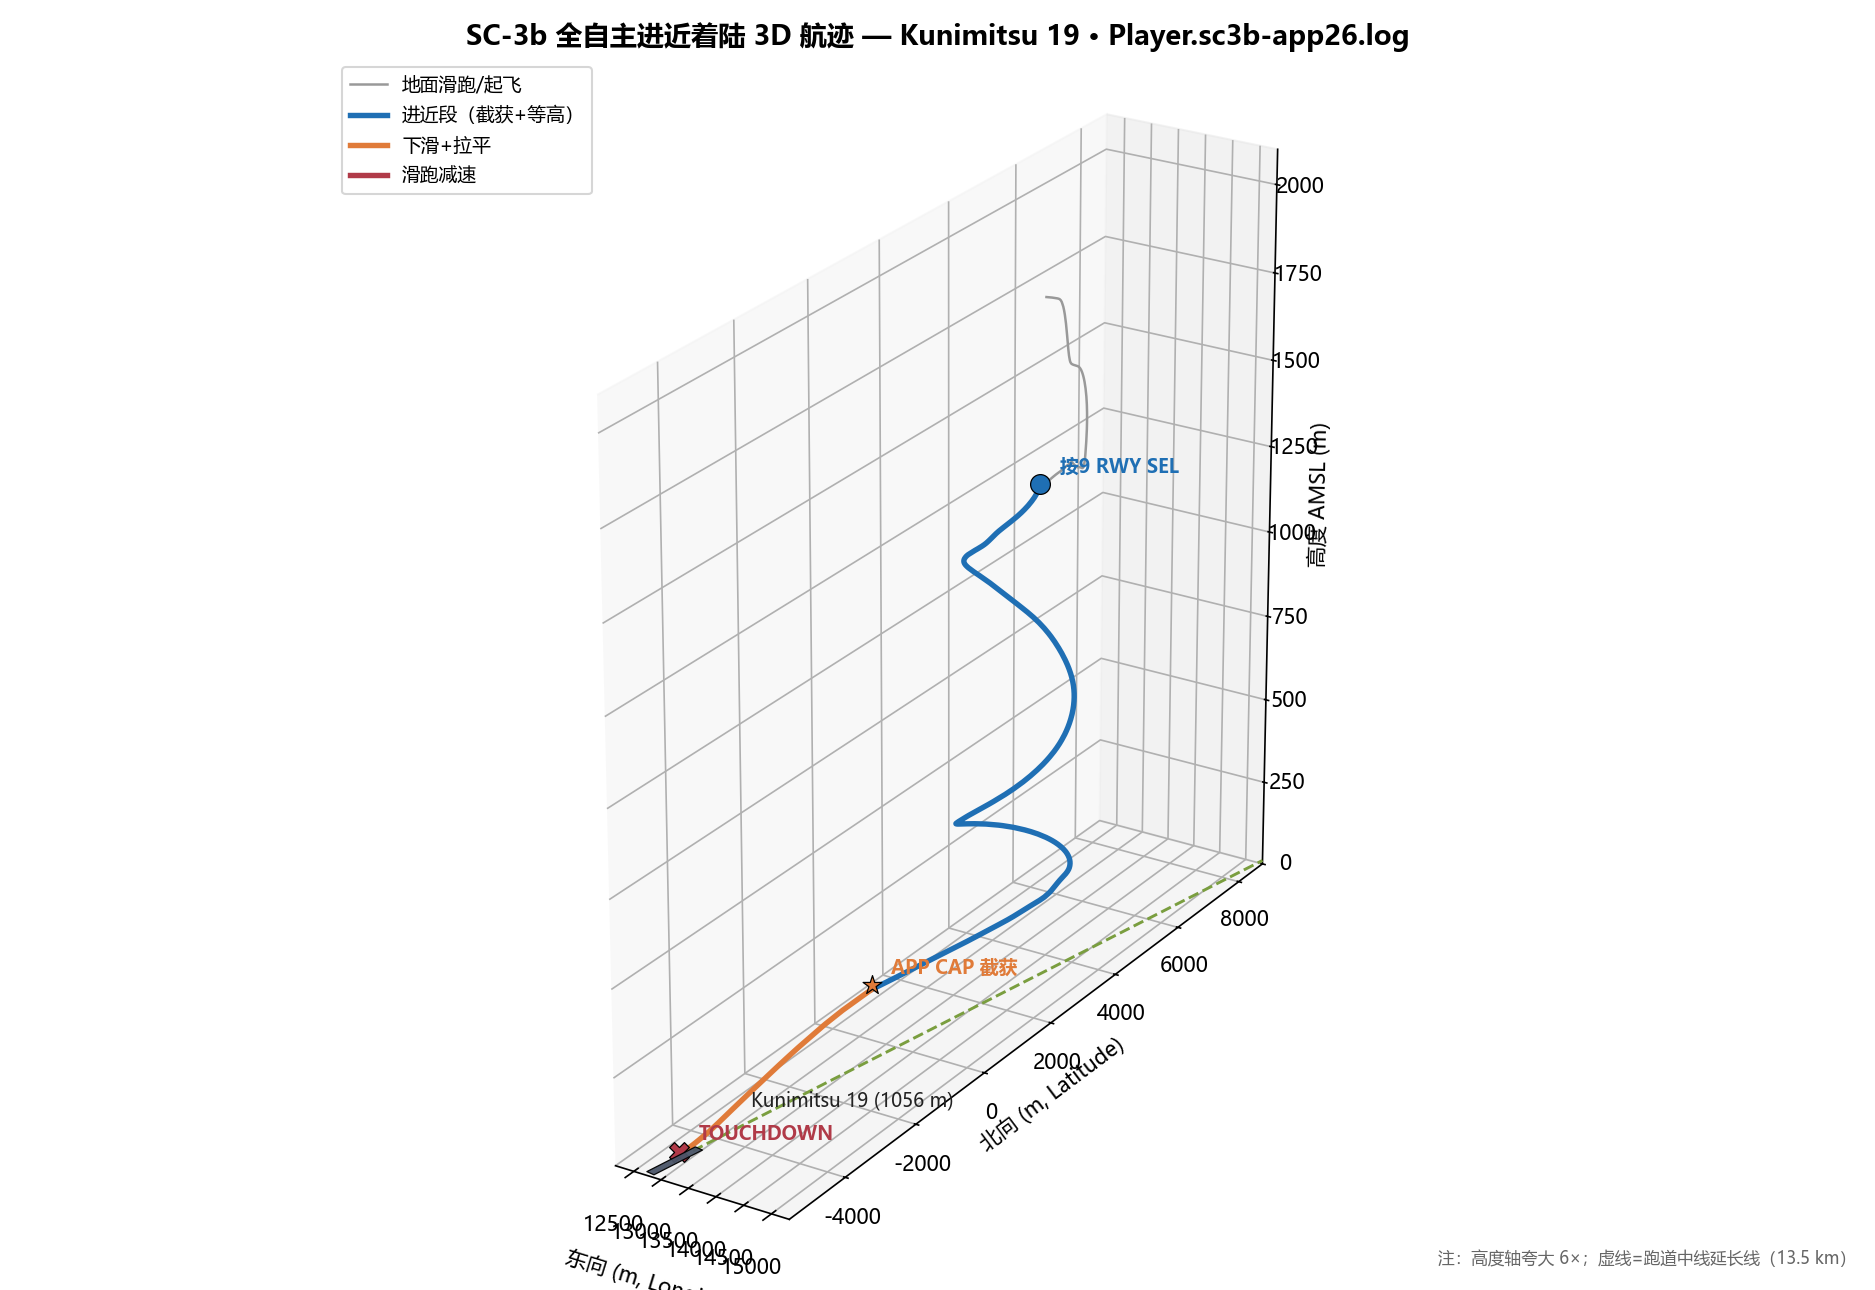
\includegraphics[width=0.98\textwidth]{sc3b-track3d-sc3b-app26.png}
\caption{app26（封版验证局）：1352 m/9.0 km 山区机场接管。接管第一拍入轨，一个相切圆完成全部消高，切点零转弯并入延长线，沿中线 4 km 后 FAF 截获、下滑、接地停稳，全程零人工接管。}\label{fig:app26}
\end{figure}

\section{遗留项}
\begin{enumerate}
\item 触地签名对软着陆（45--51 m/s、无明显俯仰冲击）仍误报 MISMATCH，属阈值问题，不影响结果判定；
\item GO-AROUND 后为直线爬升脱离，程序重加入（复飞转切线圆）已有航点机件、逻辑未接；
\item 下滑段存在约 $-30$ m 的常值侧偏（表值中线或配平静差，待标定局）；
\item 风向不可读，选向永久为几何判据；直升机坪与弹射平台未入表；
\item Kunimitsu 进近走廊地形复杂，维持远距接管黑名单，地形保险仅为兜底。
\end{enumerate}

\section{封版结论}
SC-3b 定版 v4.48：跑道选配、进场方式与剖面规划、程序/切线圆消高、FAF 闸门与着陆链交接全部实飞闭环，并在高接管、大侧偏、反侧、山区短条等对抗性场景中零人工接管落地。课题自本日起封版，遗留项转入观察清单。

\section{封版后迭代与最终收口（v4.49--v4.68）}
封版后针对遗留项与进近品质继续迭代二十版，全部改动经实飞遥测验尸裁决，问题定性一律以数据为据。迭代归为四组：
\begin{enumerate}
\item \textbf{复飞与程序重加入}（遗留项二）：复飞爬高后自动重建进场程序并二次截获的全链接线（v4.49）；复飞即收轮、放轮门修正；主动复飞判据（稳定进近门 1.5 km 未建立即 UNSTABLE、下滑离线闸收紧至侧偏 150 m/近段 90 m 与航向差 20°，v4.61）；复飞专用左航线（v4.62）与重加入门槛对实测爬升平台表（v4.60）。
\item \textbf{横向收敛结构}：滚转通道由"航向误差直出杆"（杆$\to$坡度$\to$航向双积分，实测极限环：坡度驻留 51--66°、滚转率 $\pm35^\circ$/s 方波）改为\textbf{坡度内环串级}
\begin{equation}
\varphi_c=\mathrm{clamp}\!\bigl(1.5\,\dot\psi_f-\varepsilon,\ \pm55^\circ\bigr),\qquad
\delta_a=\mathrm{clamp}\!\bigl(-0.010(\varphi_c-\varphi)+0.004\,p,\ \pm0.45\bigr),
\end{equation}
误差逼近目标时误差项自动反号，结构上实现提前收杆（v4.65）；转弯半径由四局分箱实测定标为 $r=V^2/13.5$（50° 坡档），程序拐角进一触发改为切点提前量 $r\tan(\Delta\psi/2)$（v4.66）；收线律加侧偏率微分项 $l_{\mathrm{eff}}=l+2.5\,\dot l$，快速逼近时切入角自动收小甚至反向预偏（v4.68）。
\item \textbf{能量管理与爬升性能}：俯仰泵振经帧率锁步实验定性为采样极限环（振峰 $f_s/6$），以 1 Hz 杆指令低通根除（v4.54）；能量爬升态阈值加回差（55 m 入/25 m 出）消除态机自激振荡（v4.65）；油门由 bang-bang 改比例斜坡并按执行器纯滞后（5--8 s）放慢环路带宽（v4.63--4.65）；爬升姿态律按操作者实测全速域爬升卡（$+17.9^\circ$/46 m/s $\to$ 持续 $+10.4$ m/s）重锚为
\begin{equation}
\theta_c=\mathrm{clamp}\!\bigl(0.9\,(V-52),\ -2^\circ,\ 16^\circ\bigr),
\end{equation}
平衡点 64.5 m/s、预期爬升率 6--8 m/s，慢于 52 m/s 自动压头保命（v4.68）。
\item \textbf{纵向几何与判定}：下滑油门收光、拉平窗等封版特性维持；瞄准点由跑道头内移 250 m 改为前移 250 m，以实测拉平尾段漂距（约 510 m）折算，使名义接地点落入跑道前四分之一（v4.66--4.67）；触地判定门限与瞄准点常数联动，消除历史硬编码。
\end{enumerate}

\subsection{最终验收架次}
定版 v4.68 于同场完成两架次验收（其间操作者另飞的调试架次不计）：
\begin{itemize}
\item \textbf{架次 A（Cochran 22L）}：约 4.5 km 直接进近，截获时侧偏 $+63$ m，全程侧偏无一次符号穿越（对比 v4.65 前 43° 穿越角/214 m 过冲的 S 弯），接地 $+165$ m（前四分之一），触地签名 stable/jerk 双项通过；
\item \textbf{架次 B（Kunimitsu 19，山区机场）}：1524 m 高、8.9 km 外接管，程序进场加三个切线圆消高，释放截获后首次下滑因航向偏差 20° 触发离线闸复飞；复飞段持续爬升率中值 $+9.4$ m/s（90 分位 $+10.8$，目标 4--9 m/s 达标），自动重入左航线二次截获（$l=-20$ m）、下滑、接地停稳，触地签名双项通过。该机场此前因走廊地形列入远距接管黑名单，本架次为山区高接管全链首次完整通过。
\end{itemize}
两架次 3D 航迹见图 \ref{fig:a51A}、\ref{fig:a51B}。

\begin{figure}[htbp]\centering
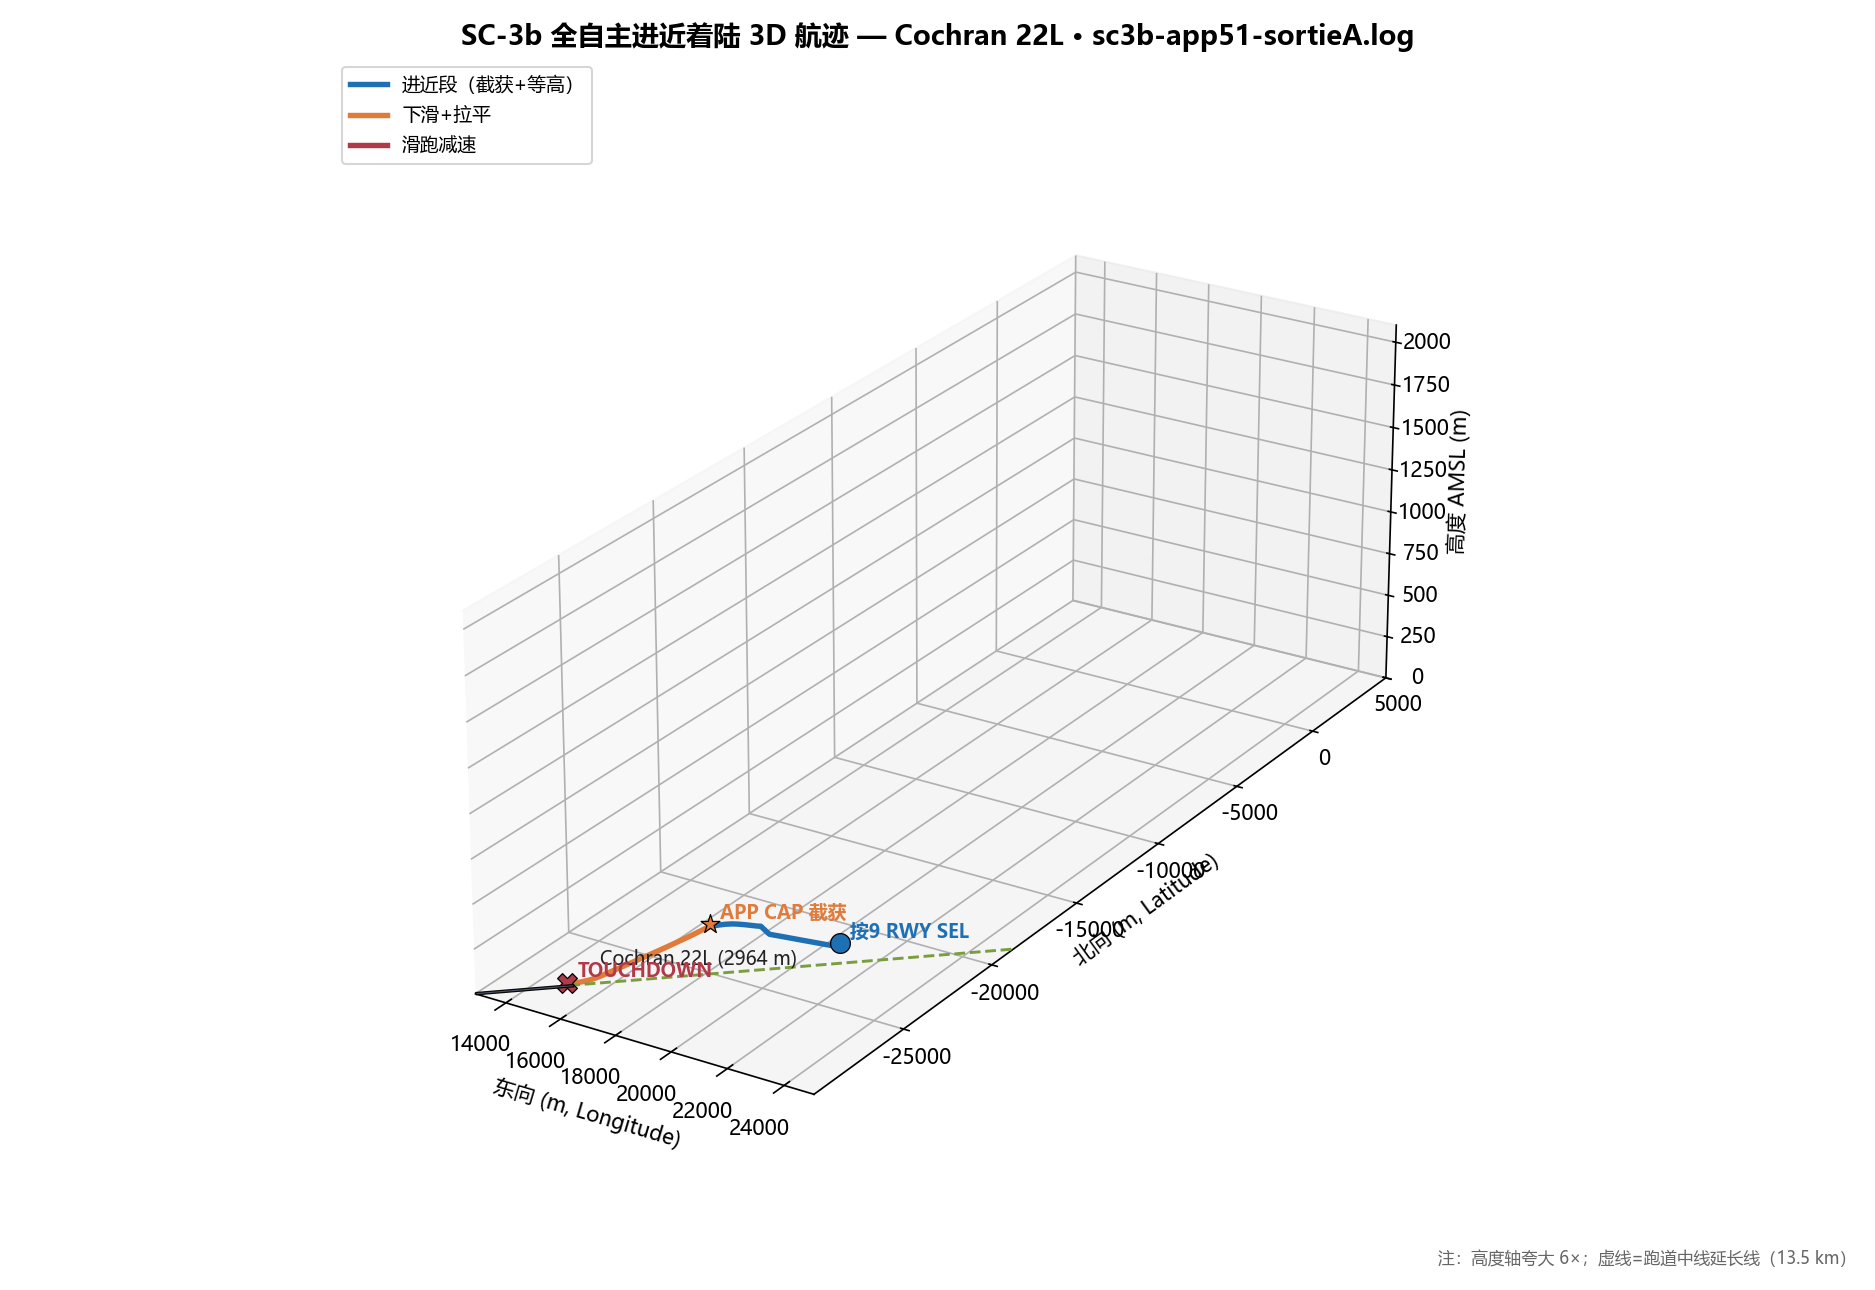
\includegraphics[width=0.98\textwidth]{sc3b-track3d-sc3b-app51-sortieA.png}
\caption{架次 A：Cochran 22L 直接进近，一次成型收线，接地 $+165$ m。}
\label{fig:a51A}
\end{figure}

\begin{figure}[htbp]\centering
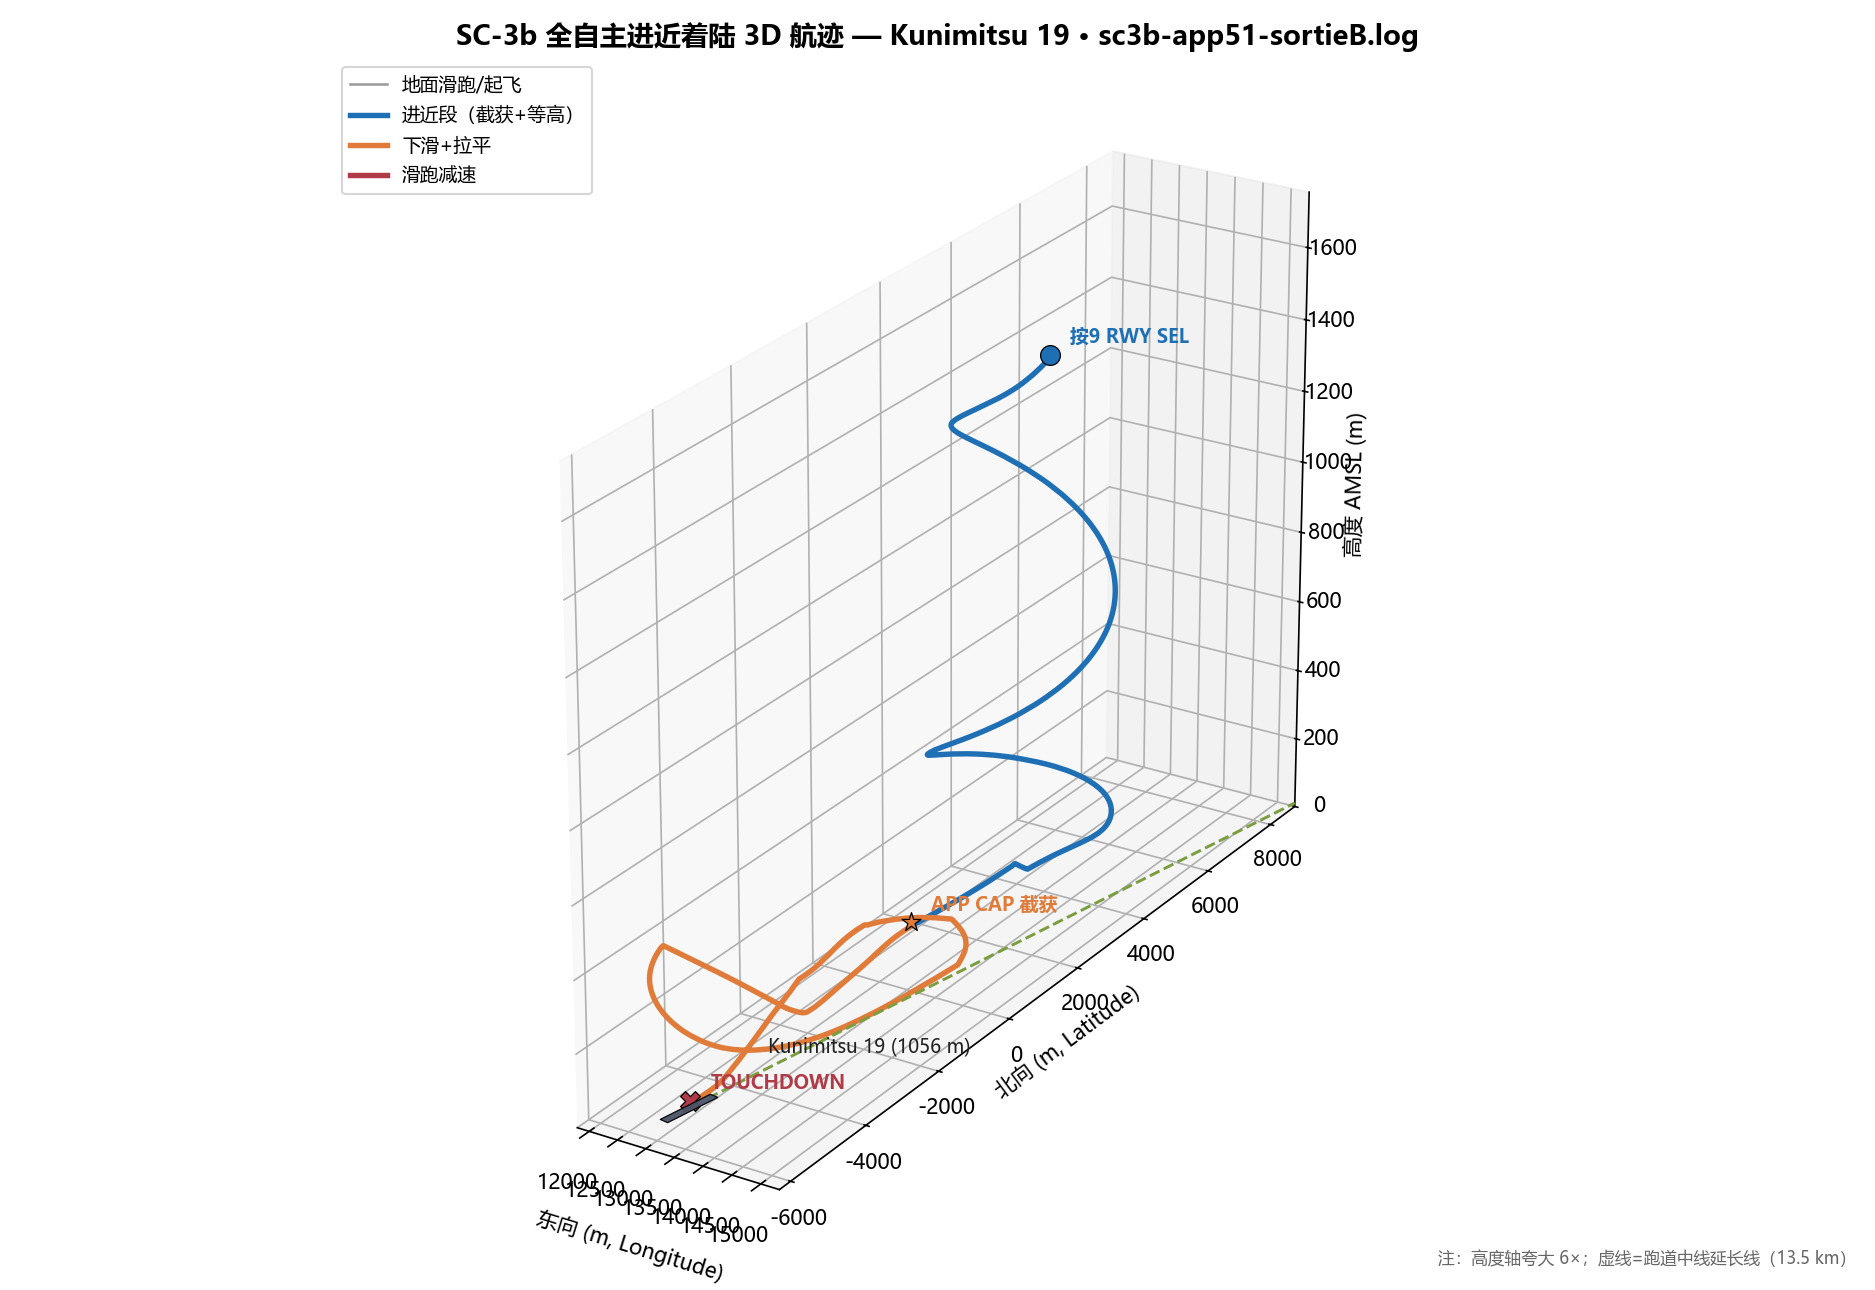
\includegraphics[width=0.98\textwidth]{sc3b-track3d-sc3b-app51-sortieB.png}
\caption{架次 B：Kunimitsu 19 山区机场 1524 m 高接管。三圈切线消高、首次下滑复飞（爬升率中值 $+9.4$ m/s）、左航线重入、二次截获接地停稳，全程零人工接管。}
\label{fig:a51B}
\end{figure}

\subsection{收口结论}
封版遗留五项至此：触地签名误报已修（两架次双项通过）；复飞程序重加入已闭环（架次 B 全链）；常值侧偏经六局离线复核判为无偏（免标定）；风向不可读维持几何选向不变；Kunimitsu 黑名单经实飞解除。SC-3b 版本冻结点由 v4.48 更新为 \textbf{v4.68}，本课题收口。

\end{document}
